% -*- TeX -*- -*- FR -*-
\documentclass[francais,letterpaper]{uds-article}

%-----------------------------------------------------------------------------
%----- Identification des packages n�cessaires
%-----------------------------------------------------------------------------

\usepackage{babel}
\usepackage[latin1]{inputenc}
%\usepackage{udstitle,dfd}
%\newcommand{\diamant}{Diamant}
\setlength{\oddsidemargin}{0.25in}
\setlength{\evensidemargin}{0.25in}
\setlength{\textwidth}{6.0in}
%\setlength{\parskip}{0.2in}
\newcounter{auxcounter}
\renewcommand{\baselinestretch}{1.5}
\setlength{\parskip}{1.5ex plus0.5ex minus0ex}

\newcommand{\ints}{\renewcommand{\baselinestretch}{1.0}\small \normalsize}
\newcommand{\intm}{\renewcommand{\baselinestretch}{1.5}\small \normalsize}
\newcommand{\intd}{\renewcommand{\baselinestretch}{2.0}\small \normalsize}


\newcommand{\bi}{\begin{itemize}}
\newcommand{\ei}{\end{itemize}}
\newcommand{\be}{\begin{enumerate}}
\newcommand{\ee}{\end{enumerate}}
\newcommand{\bd}{\begin{description}}
\newcommand{\ed}{\end{description}}



\newcommand{\bv}{\verb}

\newcommand{\bve}{\verb*}

\newcommand{\brun}{\noindent $\triangleright$}
\newcommand{\erun}{$\triangleleft$}

\newcommand{\ang}{\textsf}
\newcommand{\key}{\textsf}
\newcommand{\ita}{\textit}
\newcommand{\bld}{\textbf}
\newcommand{\dos}{\textsc}
\newcommand{\pro}{\texttt}

\newcommand{\diamant}{DIAMANT}
\newcommand{\dia}{DIAMANT 1.0}
\newcommand{\dx}{DIAMANT 1.5}
\newcommand{\saphir}{SAPHIR}
\newcommand{\sig}{SIG}

%-----------------------------------------------------------------------------
%----- Page Titre
%-----------------------------------------------------------------------------

\Titre{Mod�lisation des donn�es \\
et l'implementation de l'importation s�lective\\
Diamant 2.0}
\Logo{Images/logoDX.eps}
\Auteurs{Domingo Palao et\\
Ruben Gonzalez-Rubio \\
Mis-�-jour : 12 mai 2003}

\Date{\today}

%-----------------------------------------------------------------------------
%----- Identification des fichiers des pages pr�liminaires et bibliographique
%-----------------------------------------------------------------------------

\FichierResume{Inputs/resume}
\FichierRemerciements{}
\FichierGlossaire{} % \FichierLexique est �quivalent
\FichiersBibliographie{udsplain}{Inputs/bibDiamant,Inputs/bib2}

%-----------------------------------------------------------------------------
%----- Le document
%-----------------------------------------------------------------------------

\includeonly{Inputs/resume}

\begin{document}
\begin{articleDX}

\chapter{Le flot d'information}

Pour mieux comprendre la sp�cification d'un syst�me il faut
d'abord comprendre le flot que l'information suit. Ainsi que tous
les transformations que les donn�es passent pour devenir
information utile. Ce chapitre pr�sente la cheminement et les
transformations des donn�es.

C'est vrai que dans un syst�me de production d'horaires
l'information doit suivre un certain chemin qui modifie les
donn�es, � vrai dire, c'est le changement de l'information qui
permet � l'information d'acqu�rir une valeur ajout�e, mais ces
changements comportent des risques qu'il faut savoir controller.
Il faut pour tant, les syst�mes d'information capables d'encadrer
les utilisateurs pour faire les changements de la mani�re
appropri�e et contr�l�e, pour �viter qu'ils introduisent des
nouveaux erreurs chaque fois qu'ils utilisent un logiciel.

Pour commencer, dans la figure\ref{flot1} nous montrons d'une
mani�re simplifi�e le flot d'information. Nous montrons aussi les
entit�s participantes dans le processus, ces entit�s jouent chaque
une un r�le.

Les entit�s:
\begin{description}
\item[Serveur de l'Unit� d'administration externe.]Dans
l'environnement d�finie � notre syst�me, nous avons contact avec
une entit� externe qui g�re l'information acad�mique de
l'Universit�. Elle utilise une base de donn�es pour enregistrer
ses informations. Nous avons besoin d'interagir avec cette unit�,
l'�change d'information est bidirectional, elle doit nous envoyer
un ou plusieurs fichiers dans format texte ou XML avec
l'information de d�part pour la production des horaires, et nous
allons envoyer � la fin du processus les r�sultats de la
production des horaires.

Cette entit� a certaines r�gles qu'il faut respecter pour pouvoir
recevoir et envoyer les donn�es. Dans notre cas particuli�re, il
s'agit d'une entit� tr�s rigide o� les changements sont difficiles
� faire. C'est pourquoi il nous faut un grand niveau d'adaptation
dans le c�t� de notre interface pour s'adapter � cette entit� mais
aussi pour rester assez ouverte pour accueillir les donn�es
d'entr� d'autres entit�s.

\item[Base de donn�es.]C'est ici que nous allons enregistrer les
donn�es n�cessaires pour la creation des horaires. Nous allons
utiliser certaines relationes comme une "m�moire tampon" dans
laquelle nous allons enregistrer les donn�es bruts, c'est-�-dire,
tels qu'elles sont re�ues du serveur de l'unit� d'administration
externe. Ces donn�es peuvent avoir des erreurs dans la
construction de chaque donn�e, c'est pour cela qu'il faut
appliquer un filtrage. Ce filtrage consiste en valider les donn�es
pour les laisser conformes � une structure de base de donn�es
relationnelle normalis� ant�rieurement. Une fois que les donn�es
sont filtr�es, nous allons utiliser une deuxi�me partie de la base
de donn�es pour stocker ces donn�es filtr�es et corrig�es qui sont
pr�ts pour l'exploitation de notre application de creation
d'horaires. Chaque fois que des nouvelles donn�es arrivent, il
faut appliquer le filtrage pour valider la coherence de
l'information.

\item[Diamant.]Il s'agit de notre logiciel de cr�ation d'horaires,
il est param�trable et adaptable pour la cr�ation d'horaires de
cours, examens et autres types d'horaires. Il re�oit un ou
plusieurs fichiers d'entr�e pour cr�er les horaires et il retourne
un ou plusieurs fichiers de donn�es avec l'information de
l'horaire.
\end{description}

\begin{figure}[h]
   \centering{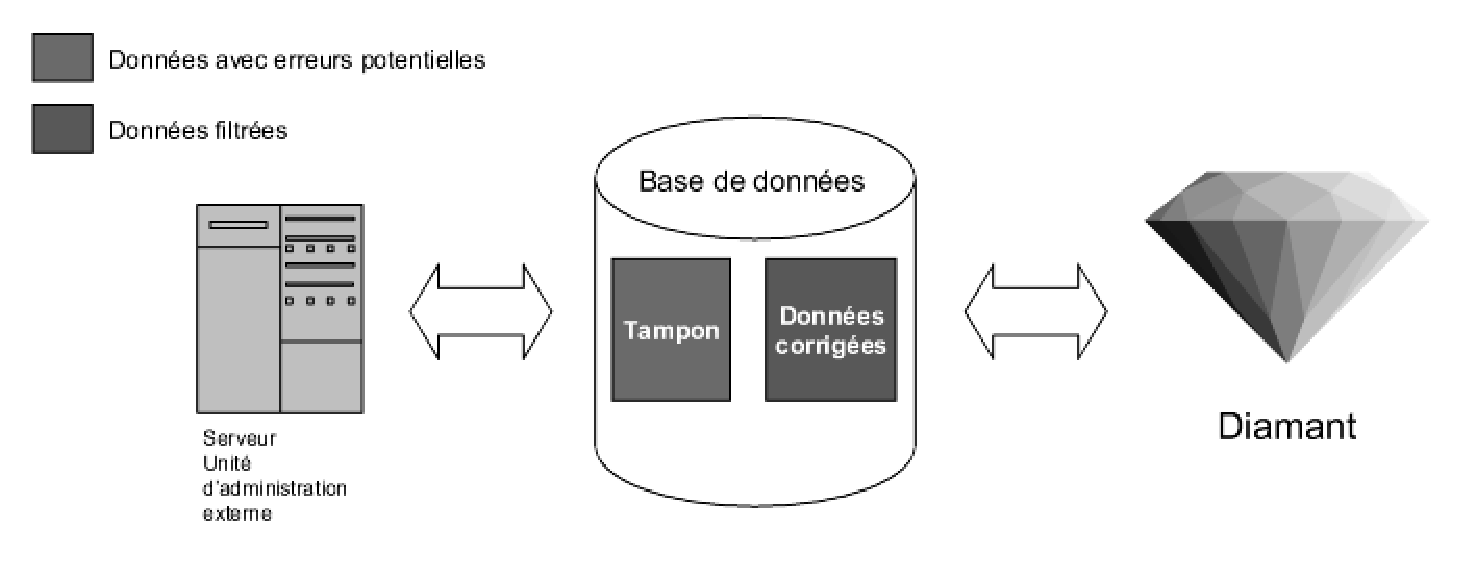
\includegraphics[width=1\textwidth]{Images/flot1.eps}}
   \caption{\emph{Le flot de l'information, vision simplifi�e.}}
   \label{flot1}
\end{figure}


Une fois que nous avons compris le flot d'information initial,
nous allons le d�tailler. Pour montrer le chemin d�taill�e que
l'information traverse dans le syst�me, nous utilisons la figure
\ref{flot2}. Dans cette figure nous avons marqu� en couleur verte
les actions qui travaillent avec des donn�es d'entr�e ou sortie de
notre syst�me, nous avons isol� le syst�me � ce partie qui g�re la
base de donn�es. En rouge nous avons laisse les donn�es qui ont
potentiellement des erreurs et qu'il faut v�rifier. En bleu nous
avons les donn�es qui sont d�j� filtr�es. Nous allons expliquer
chaque action~:


\begin{figure}[h]
\centering{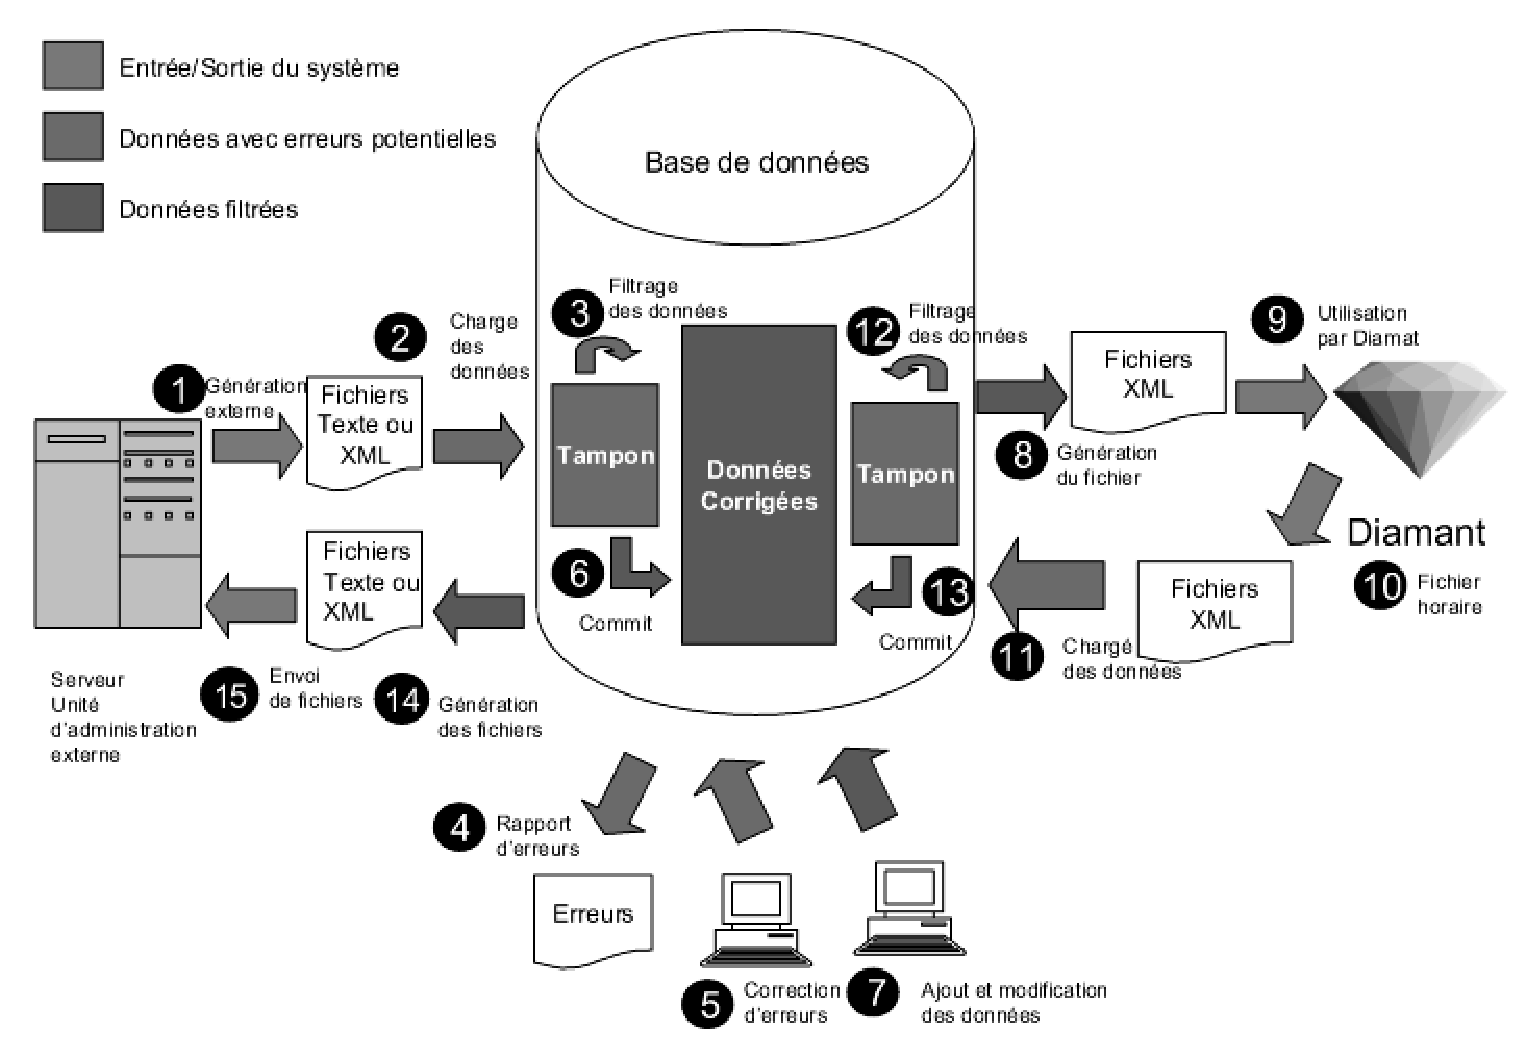
\includegraphics[width=1\textwidth]{Images/flot2.eps}}
\caption{\emph{Le flot de l'information.}} \label{flot2}
\end{figure}

\begin{description}
\item[1. G�n�ration externe.]Il y a certaines donn�es qui sont
g�n�r�es par le syst�me externe que nous avons appel� "Unit�
d'administration Externe". Cette entit� est responsable
d'administrer l'information acad�mique de l'Universit� et elle
g�nere certaines donn�es que nous allons utiliser pour la cr�ation
des horaires. L'�change de donn�es est faite � l'aide de certains
fichiers qui sont cr�es par un "job", qui est un processus
informatis� precise. Les fichiers peuvent venir en format texte ou
bien en format XML, c'est pourquoi notre syst�me doit �tre capable
de ma�triser les deux formats. Nous allons analyser la structure
de ces fichiers plus tard.

\item[2. Charge de donn�es.]Pour pouvoir modifier et mieux g�rer
les donn�es nous pensons que la meilleure outil est un syst�me de
base de donn�es, parce que ce syst�me est con�ue pour faciliter
l'acc�s et les modification � l'information. Dans une premi�re
�tape nous allons enregistrer les donn�es bruts, c'est-�-dire,
tels qu'ils sont re�ues dans quelques relations temporaires de la
base de donn�es que nous allons appel�es "tampon". Tous les
actions de filtrage et correction d'erreurs sont faites dans cette
partie de la base de donn�es.

\item[3. Filtrage de donn�es.]Dans l'�tape pr�c�dente nous avons
charg� les donn�es dans la base de donn�es, mais nous ne
connaissons pas l'�tat de ces donn�es. Par experience, nous savons
que la plupart des erreurs dans un logiciel sont attach�es aux
erreurs dans la composition des donn�es. Pour assurer la propret�
et la coherence des donn�es il va falloir appliquer un processus
de filtrage, c'est-�-dire, nous prenons les donn�es bruts et nous
faisons certains v�rifications de l'int�grit� et la coherence du
format. Tous les r�sultats du filtrage restent dans la partie
"tampon" de la base de donn�es.

\item[4. Rapport d'erreurs.]Une fois que nous avons appliqu� le
filtre des donn�es, il faut cr�er un rapport d'erreurs. Ce
document nous montr� tous les anomalies trouv�es dans les donn�es
re�ues, il est une outil importante pour l'�tape suivante.

\item[5. Correction d'erreurs.]Avec l'aide du rapport d'erreurs il
y a un utilisateur qui devra r�aliser les changements n�cessaires
pour corriger les erreurs. Une fois faites les corrections,
l'utilisateur peut re-faire les pas 3, 4 et 5, jusqu'au point
qu'il n'y aie plus d'erreurs, ou les erreurs soient minimes.

\item[6. Commit.]Une fois qu'il n'y a pas d'erreurs dans le
rapport d'erreurs, l'utilisateur peut executer la commande
"Commit", qui va transf�rer les donn�es de la partie "Tampon" de
la base de donn�es � la partie des "Donn�es corrig�es". Ces
donn�es serviront � la cr�ation des horaires.

\item[7. Ajout et modification des donn�es.]Si l'utilisateur
consid�re qu'il faut modifier certaines donn�es avant de cr�er
l'horaire il doit utiliser une interface qui lui permettra cette
activit�. Il peut ajouter certains donn�es, modifier quelques
autres, et m�me effacer quelques donn�es. Pour ces modifications
il y a certains r�gles � accomplir.

\item[8. Generation du fichier.]Avec les donn�es dans la partie
des "donn�es corrig�es" de la base de donn�es, l'utilisateur peut
cr�er un fichier en format XML avec toutes les donn�es n�cessaires
pour l'operation du logiciel \diamant{}, ce fichier tiens en
consideration tous les donn�es ajout�es, ou modifies dans la base
de donn�es.

\item[9. Utilisation par \diamant{}.]Avec les fichiers qu'il a
cr�e dans l'�tape 8, l'utilisateur est capable de cr�er son
horaire. Des fois, l'utilisateur qui participe dans cette �tape
est quelqu'un diff�rente de l'utilisateur qui a fait la saisie des
donn�es.

\item[10. Fichier horaire.]Une fois que le logiciel \diamant{} a
�t� ex�cut� et l'horaire cr�e, il faut g�n�rer un fichier sortie
avec les donn�es de l'horaire. Ce fichier est cr�e en utilisant le
format XML.

\item[11. Charge de donn�es.]Avec l'execution de \diamant{}, il y
a certains donn�es qui sont modifies. Pour assurer la coherence de
l'information il faut les charger dans la base de donn�es. Mais,
il faut faire attention, parce que ne sont pas toutes les donn�es
qui ont �t� modifies. C'est pourquoi il faut appliquer un
processus d'importation selective, les donn�es � charger sont
stockes dans la partie m�moire "Tampon2" de notre base de donn�es.

\item[12. Filtrage de donn�es.] �tant donn�e que nous voulons
introduire des nouvelles donn�es � la base de donn�es, il faut
toujours v�rifier la validit� de ces donn�es, c'est pourquoi nous
allons appliquer ici les filtres n�cessaires pour assurer la
coherence des donn�es.

\item[13. Commit.]S'il n'y a pas d'erreurs dans le filtrage des
donn�es, nous pouvons appliquer "commit" � l'information et passer
l'information � la section des "Donn�es Corrig�es".

\item[14. Generation des fichiers.]Pour retourner l'information �
l'Unit� d'Administration externe, il faut g�n�rer un ou plusieurs
fichiers en format texte ou XML contenant les modifications �
l'information de base ainsi que l'information concernant �
l'horaire qui a �t� cr�e. Dans cette �tape il faut cr�er ces
fichiers.

\item[15. Envoi des fichiers.]Une fois que le ou les fichiers sont
cr�es, il faut les envoyer � l'Unit� d'administration externe.
Avec cette activit� le cycle de cr�ation d'un horaire est termin�.

\end{description}


\appendix
%%\chapter{Description des champs pour \diamant{} 1.5}\label{fields}

\begin{table}[h]
    \begin{tabular}{*{5}{|c}|} \hline
           \itshape Champ & \itshape �l�ment Diamant & \itshape  Description& \itshape Type \footnotemark[1] & \itshape Genre \footnotemark[2]\\ \hline
          Nom du local & Liste de locaux & - & A & \\ \cline{1-4}
          & Liste de locaux & - & A & \\ \cline{2-4}
          & Conflit de capa de locaux & Recalculer les conflits & C & \\ \cline{2-4}
          \raisebox{3.0ex}[1pt]{Capacit�} & P�riode & Rafra�chissement de la p�riode & C & \\ \cline{1-4}
          & Liste de locaux & - & A & \\ \cline{2-4}
          &  & V�rifier si les caract�ristiques & & \\
          &  & du local sont adapt�es & & \\
          \raisebox{4.5ex}[1pt]{Liste de} & \raisebox{3.0ex}[1pt]{Warning de locaux} & � la nature du cours & \raisebox{3.0ex}[1pt]{C} &  \\ \cline{2-4}
          \raisebox{4.5ex}[1pt]{caract�ristiques} & P�riode & Rafra�chissement de la p�riode & C & \raisebox{12.0ex}[1pt]{D} \\ \hline
    \end{tabular}
    \caption{\emph{Fichier de locaux} }
    \label{tableLocaux}
\end{table}
\footnotetext[1]{A: champs affect� - C: champs calcul�} \footnotetext[2]{S: champs statique (immuable) - D: champs dynamique (modifiable)}

\begin{table}[h]
    \begin{tabular}{*{5}{|c}|} \hline
          \itshape Champ & \itshape �l�ment Diamant & \itshape Description & \itshape Type \footnotemark[1] & \itshape Genre \footnotemark[2]\\ \hline
          Instructeur ID(nom) & Liste de professeurs & - & A & S \\ \hline
          & Liste de disp. de profs. & - & A & \\ \cline{2-4}
          & Conflit de disp. de profs. & Recalculer les conflits & C & \\ \cline{2-4}
          \raisebox{3.0ex}[1pt]{Disponibilit�} & P�riode & Rafra�chissement de p�riode & C & \raisebox{3.0ex}[1pt]{D} \\\hline
    \end{tabular}
    \caption{\emph{Fichier de Enseignants}}
    \label{tableEnseignants}
\end{table}

\begin{table}[h]
    \begin{tabular}{*{5}{|c}|} \hline
          \itshape Champ & \itshape �l�ment Diamant & \itshape Description & \itshape Type \footnotemark[1] & \itshape Genre \footnotemark[2]\\ \hline
          Matricule & & - & & S \\ \cline{1-1} \cline{3-3} \cline{5-5}
          Nom et pr�nom & & - & & S \\ \cline{1-1} \cline{3-3} \cline{5-5}
          Sexe & & - & & D \\ \cline{1-1} \cline{3-3} \cline{5-5}
          �tat & \raisebox{4.0ex}[1pt]{Liste d'�tudiants} & - & \raisebox{4.0ex}[1pt]{A} & D \\ \hline
          �tudiant.Activit�ID & & - & & \\ \cline{1-1} \cline{3-3}
          �tudiant.Activit�Nature & \raisebox{1.0ex}[1pt]{Conflits d'�tudiants et} & - & &  \\ \cline{1-1} \cline{3-3}
          �tudiant.Num�roGroupe & \raisebox{1.0ex}[1pt]{Conflits de capacit� de locaux} & - & \raisebox{3.0ex}[1pt]{C} & \raisebox{3.0ex}[1pt]{D} \\ \cline{1-1} \hline
    \end{tabular}
    \caption{\emph{Fichier d'�tudiants}}
    \label{tableEtudiants}
\end{table}


\begin{table}[h]
    \begin{tabular}{*{5}{|c}|} \hline
          \itshape Champ & \itshape �l�ment Diamant & \itshape Description & \itshape Type & \itshape Genre\\ \hline \hline
          Nom d'activit� & Liste d'activit�s & - & A & S \\ \hline
          & Liste d'activit�s & - & A & \\ \cline{2-4}
          & Conflits de locaux & Recalculer les conflits & & \\ \cline{2-2}
          & Conflits de disp. de profs. & si les activit�s sont d�j� & & \\ \cline{2-2}
          \raisebox{4.5ex}[1pt]{Include} & Conflit d'�tudiants & plac�es dans la grille & \raisebox{3.0ex}[1pt]{C} & \raisebox{4.5ex}[1pt]{D} \\ \hline
          Session & Liste d'activit�s & - & A & D \\ \hline
          & Liste de sous-activit�s & - & A & \\ \cline{2-4}
          & Liste d'activit�s & - & A & \\ \cline{2-4}
          & & Dans le cas o� il y a eu un & & \\
          & \raisebox{1.5ex}[1pt]{Warning de locaux} & changement de nature & \raisebox{1.5ex}[1pt]{C} & \\ \cline{2-4}
          & & Dans le cas o� il y a eu une & & \\
          \raisebox{7.0ex}[1pt]{Sous-Activit�.Nature} & \raisebox{1.5ex}[1pt]{Tous les conflits} & insertion/suppression de nature & \raisebox{1.5ex}[1pt]{C} & \raisebox{7.5ex}[1pt]{D} \\ \hline
          & Liste de groupes & - & & \\ \cline{2-3}
          & Liste de sous-activit�s & - & & \\ \cline{2-3}
          & Liste d'activit�s & - & \raisebox{3.0ex}[1pt]{A} &  \\ \cline{2-4}
          & & Dans le cas o� il y a eu une & & \\
          \raisebox{6.0ex}[1pt]{Groupe.Num�ro} & \raisebox{1.5ex}[1pt]{Tous les conflits} & suppression de groupe & \raisebox{1.5ex}[1pt]{C} & \raisebox{6.0ex}[1pt]{S} \\ \hline
          & Liste de bloques & - & & \\ \cline{2-3}
          & Liste de groupes & - & & \\ \cline{2-3}
          & Liste de sous-activit�s & - & & \\ \cline{2-3}
          & Liste d'activit�s & - & \raisebox{4.5ex}[1pt]{A} &  \\ \cline{2-4}
          & & Dans le cas o� il y a eu une & & \\
          \raisebox{6.0ex}[1pt]{Bloque.Num�ro} & \raisebox{1.5ex}[1pt]{Tous les conflits} & suppression de bloque & \raisebox{1.5ex}[1pt]{C} & \raisebox{7.5ex}[1pt]{S} \\ \hline
          & Toutes les listes & - & A & \\ \cline{2-4}
          & Conflit de locaux & - & C & \\ \cline{2-4}
          \raisebox{3.0ex}[1pt]{Bloque.LocalID} & Warning de locaux & - & C & \raisebox{3.0ex}[1pt]{D} \\ \hline
          & Toutes les listes & - & A & \\ \cline{2-4}
          \raisebox{1.5ex}[1pt]{Bloque.P�riodeID} & Tous les conflits & - & C & \raisebox{1.5ex}[1pt]{D} \\ \hline
          & Toutes les listes & - & A & \\ \cline{2-4}
          \raisebox{1.5ex}[1pt]{Bloque.Dure�} & Tous les conflits & - & C & \raisebox{1.5ex}[1pt]{D} \\ \hline
          & Toutes les listes & - & A & \\ \cline{2-4}
          \raisebox{1.5ex}[1pt]{Bloque.Activit�Type} & Warning de locaux & - & C & \raisebox{1.5ex}[1pt]{D} \\ \hline
          & Toutes les listes & - & A & \\ \cline{2-4}
          \raisebox{1.5ex}[1pt]{Bloque.Plac�} & Tous les conflits & - & C & \raisebox{1.5ex}[1pt]{D} \\ \hline
          & Toutes les listes & - & A & \\ \cline{2-4}
          \raisebox{1.5ex}[1pt]{Bloque.Fig�} & Tous les conflits & - & C & \raisebox{1.5ex}[1pt]{D} \\ \hline
          & Toutes les listes & - & A & \\ \cline{2-4}
          \raisebox{1.5ex}[1pt]{Bloque.Instructeur} & Conflit d'instructeur & - & C & \raisebox{1.5ex}[1pt]{D} \\ \hline
    \end{tabular}
    \caption{\emph{Fichier de Cours}}
    \label{tableCours}
\end{table}


  % after \\: \hline or \cline{col0-col2} \cline{col3-col4} .

\end{articleDX}
\end{document}
